\documentclass{article}
\usepackage[utf8]{inputenc}
\usepackage{paralist}
\usepackage{subfig}
\usepackage{tabularx}
\usepackage{tikz}
\usepackage{booktabs}
\usepackage{paralist}
\usepackage{tablefootnote}

\title{CSE221 - System Profiling}
\author{Ruchir Garg (rugarg@ucsd.edu), Max Gao (magao@ucsd.edu) }
\date{October 2022}

\begin{document}

\maketitle

\section{Introduction}

Our project benchmarks various system operations and in doing so, attempts to 
approximate hardware performance at the software level. The system components
we benchmark include:
\begin{itemize}
    \item CPU Scheduling
    \item Memory
    \item Network
    \item File System
\end{itemize}

Our measurements are performed by code written in C which we compile with gnu C++=11
with various levels of optimization (level 2 by default, otherwise noted). We developed on
our local machines and executed the measurements on a bare metal server rented from an
infrastructure provider, Vultr. Work was split evenly: Ruchir laid out the initial codebase
and contributed measurement code for the CPU and Filesystem; Max contributed code to generate
measurement graphs alongside measurement code for memory and network components. 

We estimate that each team member worked a total of \textbf{X} hours.
Estimate the amount of time you spent on this project.

\section{Machine Description}
\label{sec:mach}

To minimize variability in our measurement times arising from virtualization between tenants on a 
shared physical machine, i.e. inter-tenant resource contention, we opted for a single-tenant, 
bare-metal server. 
The machine's hardware specifications are as follows:

\begin{table}[h]
    \centering
    \caption{Bare-Metal Server Specs}
	\begin{tabularx}{\linewidth}{ll}
		\toprule
        CPU Model Name & Intel E3-1270 \\
        L1 cache size & 32768 B (~ 32 KB) \\
        L2 cache size & 262144 B (~ 262 KB) \\
        L3 cache size & 8388608 B (~ 8.3 MB) \\
        Frequency (per core) & 3118.588 Mhz (~ 3 GHz) \\
        TLB0 size & 32x2MB pages \\
        TLB size & 64x4K pages \\
        \midrule

        Instruction Set & x86-64 \\
        Data & (???)  \\
        RAM & 32 GB \\
        IO Bus & (???) \\    

        \midrule
        DIsk Capacity & 240 GB \\
        RPM & N/A \\ % not available for SSD 
        Control Cache Size & N/A \\ % not available for SSD
        % \item Control Cache Size = 16384 KBytes

        \midrule
        Network Card Speed & 10000 Mbits/s \\

        \midrule
        Distribution Name & Ubuntu  \\
        Version & 22.10 \\
        Linux Kernel & 5.19.0-26-generic \\
        \bottomrule
	\end{tabularx}
    \label{fig:mach_specs}
\end{table}

\section{Methodology}

\subsection{Base Hardware Performance Measurements}

Our pre-experimental setup further reduces variability arising from intra-machine, inter-process resource 
contention. We modify the \textit{isolcpus} kernel parameter before booting to ensure that a single process 
is given exclusive use to a CPU core. Furthermore, we modify these cores' \textit{IRQ affinity} so that 
interrupts are handled by non-isolated cores. Measurement processes are then scheduled on isolated cores 
after setting their \textit{cpu affinity}.

We run each experiment, unless otherwise noted, for 100,000 iterations and calculate average times using 
the number of clock-cycles and our machine's CPU frequency (see Table \ref{fig:mach_specs}). 

%%% TODO: Add details and citations for TSC %%%

\subsubsection{CPU, Scheduling, and OS Services}

\paragraph{Measurement Overhead}

To measure the time taken by a process, we check the clock time before and after the process is complete.
To measure the the overhead of reading time, we calculate the average time taken to perform a system call over
a set of calls and estimate that the overhead to record time would be twice as much as the recorded average.

To measure the overhead time from iterating a for loop, we measure the time taken by a standalone 
operation (t) and the total time it to complete a loop (T),for which the number of iterations performed is N. 
Hence the overhead per iteration due to for loop would be $(\frac{T}{N} - t)$ 

\paragraph{Procedure Call Overhead}

To measure procedure call overhead, we schedule a process on our isolated core which executes 7 variations of a function that
prints integer arguments. Each variation accepts one additional integer argument than its preceding variation. We check the 
clock times between function calls to measure times for each variation.

\paragraph{System Call Overhead}

The isolated core will run a program that invokes a list of system calls (once per program execution to avoid cache effects) and 
output the elapsed times for each, using, again, clock time differences. We compare average system 
call time measurements against outputs of the command \textit{strace} to ensure that no significant 
discrepancies exist (though we anticipate \textit{strace} benchmarked times to be slightly higher than what our program reads. 
We compare these average times of system calls to procedure calls.

\paragraph{Task Creation Time}

On our isolated core, we will execute a C program that performs the following to measure process creation time:
\begin{compactitem}
  \item Outputs the clock time to stdout
  \item Calls fork() to spawn a child process on the same core.
  \item Child process outputs the clock time to stdout
\end{compactitem}

\noindent{}Another C program will perform the following to measure pthread creation time:
\begin{compactitem}
  \item Outputs the clock time to stdout.
  \item Calls pthread\_create() to request a kernel thread.
  \item Kernel thread outputs the clock time to stdout.
\end{compactitem}

\paragraph{Context Switch Time}

\begin{compactitem}
  \item Outputs the clock time to stdout
  \item Calls popen(subprocess)
  \item inside the subprocess output the clock time.
  \item Switch back to the master process, and output clock time.
\end{compactitem}

The difference between the times is the time to switch context $+$ task creation.
We already measured the time for task creation. Hence the context switch time is the mean of the time differences $-$ time to create task.  

\subsubsection{Memory}
\paragraph{RAM Access Time}

We measure a single integer's load time from main memory, L1, and L2 by the following procedure.


\paragraph{RAM Bandwidth}

TO WRITE
% Similar to the methodology in described in lmbench, we measure the RAM Bandwidth of our system by implementing a user-level program that 
% reads and writes aligned words to main memory. For these measurements we plan on disabling hardware-based prefetching on our machine.

\paragraph{Page Fault Service Time}

% A page fault occurs when the referenced page is not found in the main memory, on this page fault the page fault handling routine is executed. The time taken to service the page fault is is the \textbf{Page Fault Service Time}.
% A simple case here would be to map a file from disk to virtual memory with the mmap() syscall. Reading the disk contents referenced by the file descriptor will trigger a page fault.
% Similarly we can do this for a scalar value or a list of integers and calculate the latencies as a function of the page size in question to measure the \textit{Page Fault Service Time}.
% Report the time for faulting an entire page from disk (mmap is one useful mechanism). Dividing by the size of a page, how does it compare to the latency of accessing a byte from main memory?

\subsection{Network}

For all remote experiments, we run a client on our original measurement machine and a server on a machine with the same specs
located within the same city as the original. We were unable to determine if both machines were colocated within the same
rack or data center.

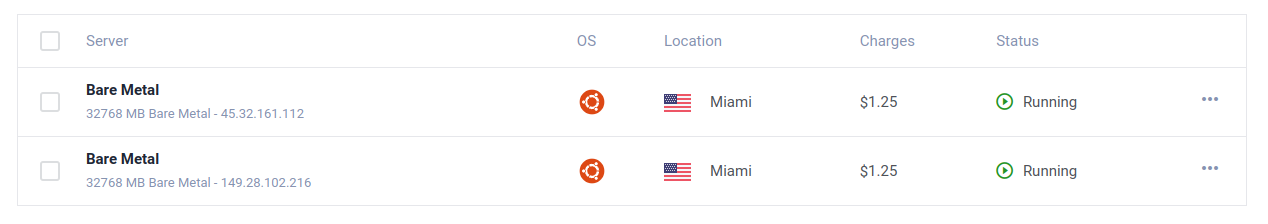
\includegraphics[width=\textwidth]{servers.png}

\subsubsection{Round trip time} 

We evaluated the Round-Trip Time (RTT) for both a TCP and ICMP request. For each protocol, we measured the RTT of packets
sent to and received over the loopback interface, i.e. the IP protocol stack is used as an interprocess communication mechanism, 
and packets sent to and received by remote host within Vultr's network.

Our local ICMP ping implementation (icmp\_loopback\_RTT.c) is a single process that sends and receives an ICMP Echo request packet 
through the same socket. We calculate the elapsed times between \textit{sendto()} and \textit{recvfrom()} system calls for each 
iteration. The remote implementation separates the sending and receiving logic into two separate processes across two cores, 
each belonging to a separate machine. 

Our local TCP implementation (tcp\_loopback\_client.c and tcp\_loopback\_server.c) comprises of two processes, each with its own 
socket bound to a different port on the loopback interface. We calculate the elapsed time between the \textit{write()} and 
\textit{read()} calls on the client process, discounting the connection setup time. We repeat the procedure for the remote
implementation (tcp\_remote\_client\_RTT.c and tcp\_remote\_server\_RTT.c) except the two processes instead execute on separate 
cores belonging to separate machines. 


% \begin{table}[h]
%     \begin{tabularx}{\linewidth}{ s {1em} *{4}{s} }
%     \toprule
% Protocol    & \multicolumn{2}{s}{Loopback RTT} 
%             & \multicolumn{2}{s}{Remote RTT} \\
%     \midrule
% ICMP   &   12  &   12  &   12  &   12 \\
% TCP    &   12  &   12  &   12  &   12 \\
%     \bottomrule
%     \end{tabularx}
% \end{table}

\subsubsection{Peak bandwidth}

We measure bandwith by sending a payload of fixed size, ~1.07GB ($2^30$ bytes). We test this over 8 different TCP payload 
lengths: 512, 1024, 2048, 4096, 8192, 16384, 32768, and 64000 (the maximum TCP payload length assuming a maximum MTU of 65536).
For each length, we send the total payload partitioned by the payload length and measure the number of cycles it took to transmit
the payload (tcp\_remote\_client\_bw.c). For simplicity sake, we calculate bandwidth over the entire window of time, though it's 
likely that there are fluctuations at smaller time intervals. 

\subsubsection{Connection overhead}

The connection overhead......
 

\section{File System}
\subsection{Size of file cache} 

Note that the file cache size is determined by the OS and will be sensitive to other load on the machine; for an application accessing lots of file system data, an OS will use a notable fraction of main memory (GBs) for the file system cache. Report results as a graph whose x-axis is the size of the file being accessed and the y-axis is the average read I/O time. Do not use a system call or utility program to determine this metric except to sanity check.

\subsection{File read time} 

Report for both sequential and random access as a function of file size. Discuss the sense in which your "sequential" access might not be sequential. Ensure that you are not measuring cached data (e.g., use the raw device interface). Report as a graph with a log/log plot with the x-axis the size of the file and y-axis the average per-block time.

\subsection{Remote file read time}

Repeat the previous experiment for a remote file system. What is the "network penalty" of accessing files over the network? You can either configure your second machine to provide remote file access, or you can perform the experiment on a department machine (e.g., APE lab). On these machines your home directory is mounted over NFS, so accessing a file under your home directory will be a remote file access (although, again, keep in mind file caching effects).

\subsection{Contention} 

Report the average time to read one file system block of data as a function of the number of processes simultaneously performing the same operation on different files on the same disk (and not in the file buffer cache).

\section{Results and Discussion}

%%%%%%%%%%%%%%%%%%%%%%%%%%%%%%%%%%%%%%
%%% CPU + Scheduling + OS Services %%%
%%%%%%%%%%%%%%%%%%%%%%%%%%%%%%%%%%%%%%
\subsection{CPU, Scheduling, and OS Services Estimates and Results}

\begin{table}[h]
    \caption{CPU, Scheduling, and OS Services Estimates and Measurements 1} \label{tab:all-CPU-1}
    \begin{tabularx}{\linewidth}{ p{10em} *{4}{p{5em}} }
    \toprule
Operation & Base Hardware Perf. & Est. Software Overhead & Pred. Time & Measured Time (Avg ms) \\
    \midrule
    Task Creation (processes) & & & & 55.318 \\
    \hline
    Task Creation (kthreads) & & & & 7.833 \\
    \hline
    Context Switch (processes) & & & & 1.384 \\
    \hline
    Context Switch (Kthreads) & & & & 1.380 \\
    \hline
    \bottomrule
    \end{tabularx}
\end{table}

\begin{table}[h]
    \caption{CPU, Scheduling, and OS Services Estimates and Measurements 2} \label{tab:all-CPU-2}
    \begin{tabularx}{\linewidth}{ p{10em} *{4}{p{5em}} }
    \toprule
Operation & Base Hardware Perf. & Est. Software Overhead & Pred. Time & Measured Time (Avg ns) \\
    \hline
    Loop Overhead & & & & 1328 \\
    \hline
    Reading Time Overhead & & & & 7514 \\
    \hline
    Procedure Call Overhead & & & & \\
    \hline
    System Call Overhead & & & & 48 \\
    \hline
    \bottomrule
    \end{tabularx}
\end{table}


%%%%%%%%%%%%%%%%%%%%%%%%%%%%%%%%%%%%%%
%%%%%%%%%%%%% Memory %%%%%%%%%%%%%%%%%
%%%%%%%%%%%%%%%%%%%%%%%%%%%%%%%%%%%%%%
\subsection{Memory Estimates and Results}

Please see attached pdfs.

%%%%%%%%%%%%%%%%%%%%%%%%%%%%%%%%%%%%%%
%%%%%%%%%%%%% Network %%%%%%%%%%%%%%%%
%%%%%%%%%%%%%%%%%%%%%%%%%%%%%%%%%%%%%%
\subsection{Network Estimates and Results}
\begin{table}[h]
    \caption{Network Measurements (* denotes sending to loopback interface)} \label{tab:all-network}
    \begin{tabularx}{\linewidth}{ p{10em} *{4}{p{5em}} }
    \toprule
Operation & Base Hardware Perf. & Est. Software Overhead & Pred. Time & Measured Time \\
    \midrule
        RTT* (ICMP) &  &  &  & 3.9ms \\
        \hline
        RTT (ICMP) &  &  &  & N/A \\
        \hline
        RTT* (TCP) &  &  &  & 14.9ms \\
        \hline
        RTT (TCP) &  &  &  &  78.3ms \\
        \hline
        Conn. Overhead* (TCP) &  &  &  & 43.7ms \\
        \hline
        Conn. Overhead (TCP) &  &  &  & 67.2 \\
        \hline
    \end{tabularx}
\end{table}

\begin{table}[h]
        \caption{Network Bandwidth Measurements (* denotes sending to loopback interface)} \label{tab:network-bw}
        \begin{tabularx}{\linewidth}{ p{10em} *{4}{p{5em}} }
        \toprule
        Operation & Base Hardware Perf. & Est. Software Overhead & Pred. Time & Measured Bandwidth (MB/s)\\
        \midrule
            Peak Bandwidth* (TCP) & N/A & N/A & N/A & 2253.56 \\
            \hline
            Peak Bandwidth (TCP) & N/A & N/A & N/A & 962.22 \\
            \hline
        \end{tabularx}
\end{table}

Though our bandwidth measurements in the remote case approaches the maximum speed reported for the 
network card on our machine (1000Mbit/s or 1.25GB/s) as we increase the payload size, a 64K payload
only yields 76\% of the theoretical hardware maximum. We did not have time to investigate the cause
for this. If we were to estimate the bandwidth, we'd establish a lower bound on the number of 
syscalls for the various phases of TCP and express bandwidth as a function of this fixed cost lower 
bound and network latency.

\begin{figure}[h]
    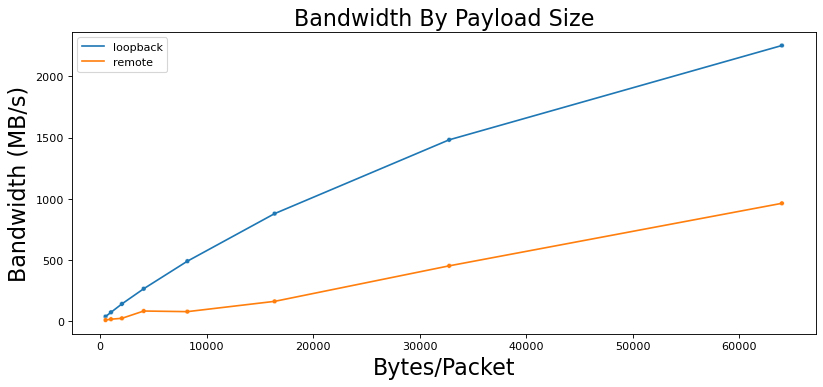
\includegraphics[width=\textwidth]{payload_bw.png}
    \label{fig:bw}
\end{figure}

\begin{figure}[h]
    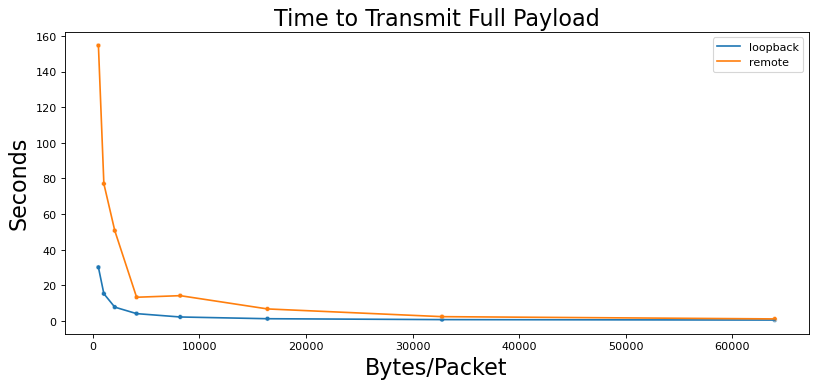
\includegraphics[width=\textwidth]{payload_transmit_time.png}
    \label{fig:transmit}
\end{figure}


%%%%%%%%%%%%%%%%%%%%%%%%%%%%%%%%%%%%%%
%%%%%%%%%%% Filesystem %%%%%%%%%%%%%%%
%%%%%%%%%%%%%%%%%%%%%%%%%%%%%%%%%%%%%%
\subsection{Filesystem Estimates and Results}

Please see attached pdfs for results.

\end{document}
